\documentclass[12pt, a4paper, twoside]{article}

%% Preamble
\usepackage{umatfgspanish}
\graphicspath{{./images/}}

\begin{document}

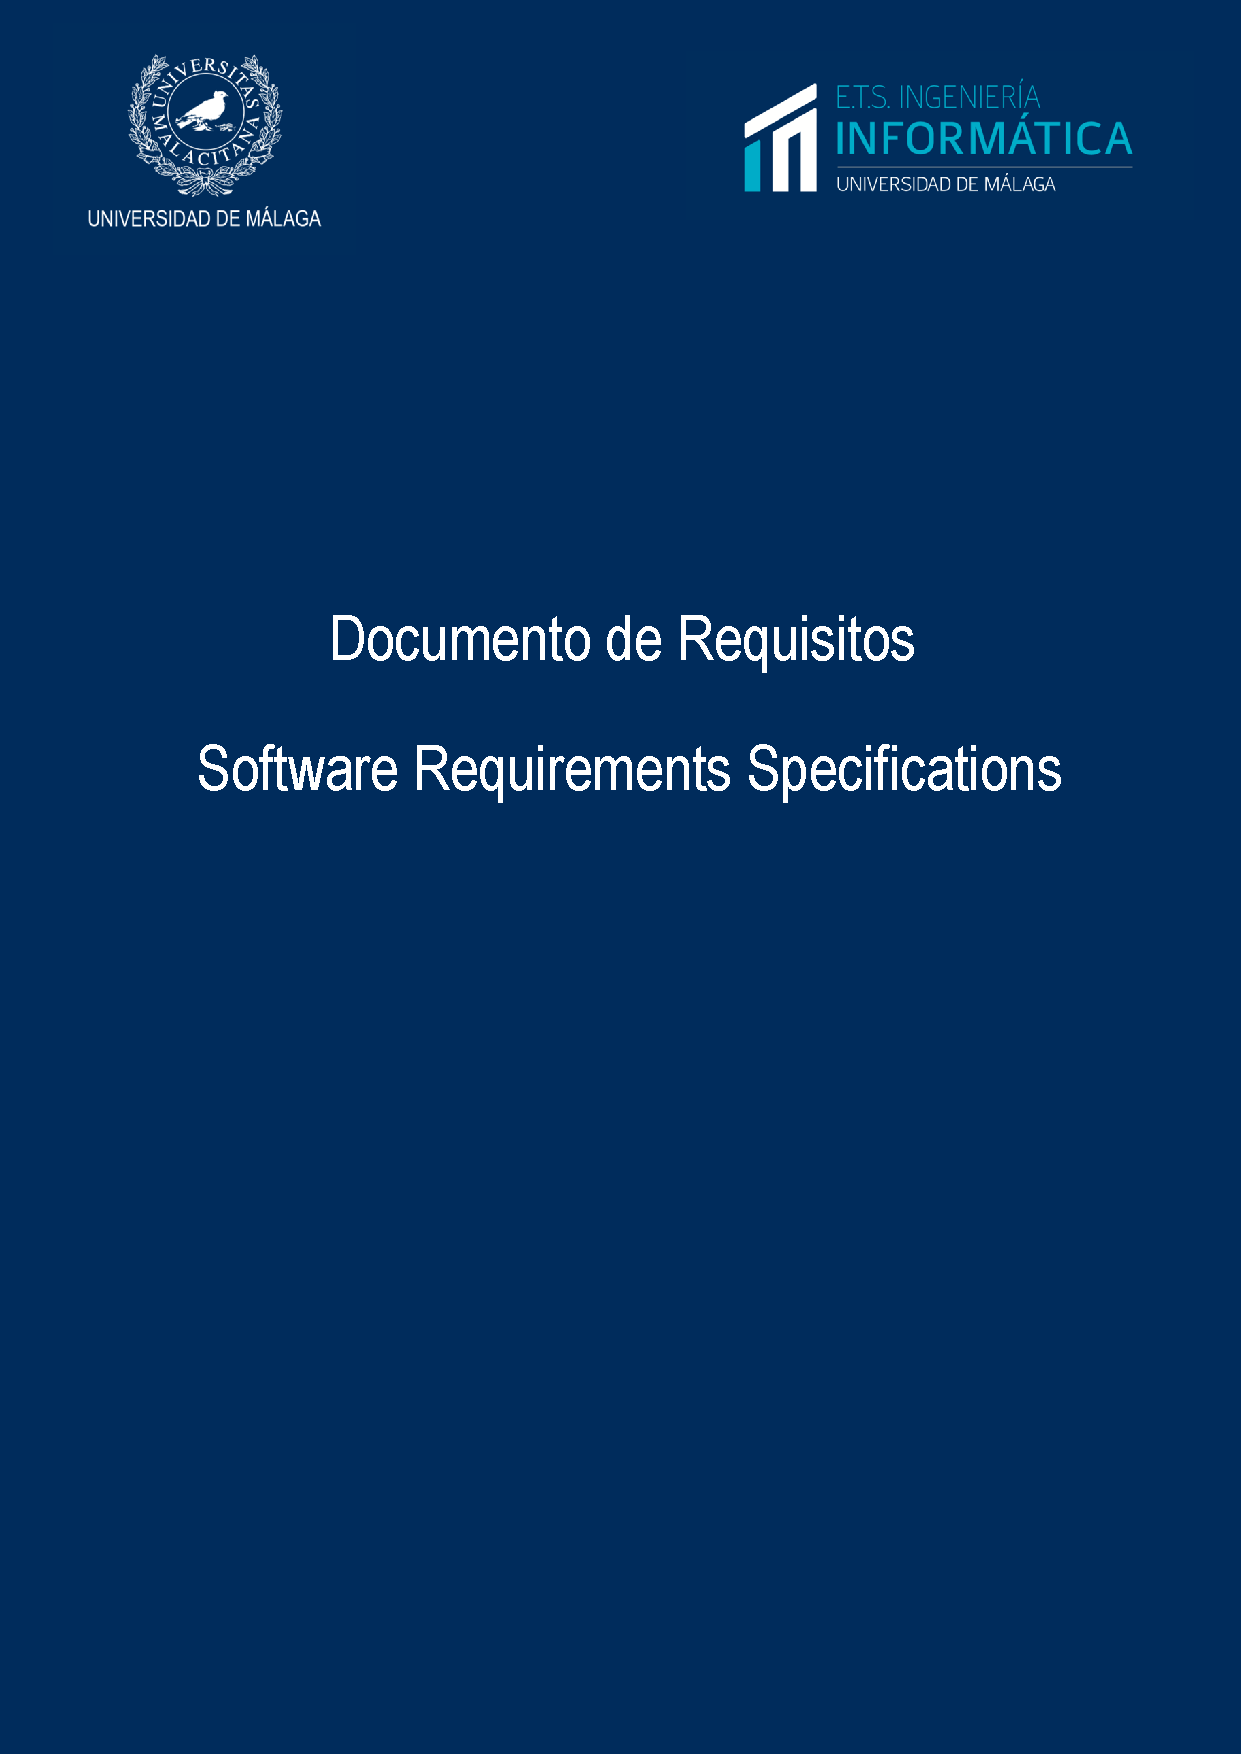
\includepdf[noautoscale=true, width=\paperwidth]{title.pdf}

\newpage

\tableofcontents

%% Sections
\section{Análisis del proyecto}
\subsection{Contextualización}
El contexto que se va a desarrollar a continuación, parte del concepto de Internet de las Cosas (IoT).
Este concepto se basa en considerar, como usuarios de internet, un conjunto de usuarios más amplio que el 
habitual. Es decir, no solo incluir a personas y a servidores, sino también tratar a cualquier objeto 
físico como un candidato a formar parte del sistema.

La consecuencia
Los resultados derivados
El potencial del IoT radica en la posibilidad

Desde que se empezó a aplicar el concepto de IoT, ha ido creciendo el números de <<cosas>> conectadas a él. 
Por ejemplo...
En los últimos  años, el uso del IoT ha aumentado exponencialmente [ENSEÑAME LO QUE TIENES].
\subsection{Problemática y oportunidades identificadas}
De acuerdo con (Estevez et al., 2021), la densidad de población que habita en las ciudades crece aceleradamente.
Se espera que para el 2030, un 60\% de las personas viva en las ciudades. 

Al existir una migración tan importante de áreas rurales a urbanos, el entorno de la
propia ciudad evoluciona más rápido y los retos a los que estas se enfrentan, o se espera que se enfrenten,
también cambian notablemente: el transporte, impacto medioambiental, salud pública, servicios, etc. Son puntos
críticos que merecen especial atención para mantener y mejorar el funcionamiento y la calidad de vida en
las urbes.

Todo esto sumado al crecimiento de las infraestructuras de telecomuncación (Banda ancha, wifi y 5G)
y a las inversiones en inteligencia artificial y big data, abren la posiblidad de aplicar la IoT como
posible solución y ofrecer mejoras a los gobiernos y ciudadanos, que ayuden a mejorar la gestión de las 
ciudades, mejoren la calidad de vida en las mismas y sean lo más respetuosas con el entorno.

Estevez E., Pardo, T., \& Scholl, J. (2021).
Smart cities and smart governance: towards the 22nd century sustainable city. Springer.


--------------------
El IoT es una tecnología relativamente reciente y son muchos los campos en los que se puede 
aplicar para sacar ventaja.

El potencial que se le puede sacar a esta red de dispositivos es muy elevado. Existen conceptos tales como:
 - IoT Orchestation
 - Fog Computing
 - 
\end{document}